% This must be in the first 5 lines to tell arXiv to use pdfLaTeX, which is strongly recommended.
\pdfoutput=1
% In particular, the hyperref package requires pdfLaTeX in order to break URLs across lines.

\documentclass[11pt]{article}

% Change "review" to "final" to generate the final (sometimes called camera-ready) version.
% Change to "preprint" to generate a non-anonymous version with page numbers.
\usepackage[final]{acl}

% Standard package includes
\usepackage{times}
\usepackage{latexsym}

% For proper rendering and hyphenation of words containing Latin characters (including in bib files)
\usepackage[T1]{fontenc}
% For Vietnamese characters
% \usepackage[T5]{fontenc}
% See https://www.latex-project.org/help/documentation/encguide.pdf for other character sets

% This assumes your files are encoded as UTF8
\usepackage[utf8]{inputenc}

% This is not strictly necessary, and may be commented out,
% but it will improve the layout of the manuscript,
% and will typically save some space.
\usepackage{microtype}

% This is also not strictly necessary, and may be commented out.
% However, it will improve the aesthetics of text in
% the typewriter font.
\usepackage{inconsolata}

%Including images in your LaTeX document requires adding
%additional package(s)
\usepackage{graphicx}
\usepackage{subcaption}

\usepackage{acronym}
\usepackage[inline]{enumitem}
\usepackage{booktabs}
\usepackage{tabularx}
% MUST BE THE LAST IMPORT
\usepackage{cleveref}

\acrodef{gnn}[GNN]{Graph Neural Network}

\newcommand{\meta}[1]{{\color{blue}#1}}

% If the title and author information does not fit in the area allocated, uncomment the following
%
%\setlength\titlebox{<dim>}
%
% and set <dim> to something 5cm or larger.

\title{Graph Neural Network Project \\
Bertinoro International Spring School (BISS) 2024}

% Author information can be set in various styles:
% For several authors from the same institution:
% \author{Martina Baiardi \and Davide Domini \and Nicolas Farabegoli \and Alessandro Petrella \and Gianni Tumedei }
%         Address line \\ ... \\ Address line}
% if the names do not fit well on one line use
%         Author 1 \\ {\bf Author 2} \\ ... \\ {\bf Author n} \\
% For authors from different institutions:
% \author{Author 1 \\ Address line \\  ... \\ Address line
%         \And  ... \And
%         Author n \\ Address line \\ ... \\ Address line}
% To start a separate ``row'' of authors use \AND, as in
% \author{Author 1 \\ Address line \\  ... \\ Address line
%         \AND
%         Author 2 \\ Address line \\ ... \\ Address line \And
%         Author 3 \\ Address line \\ ... \\ Address line}


\author{
  Martina Baiardi \\
  University of Bologna \\
  {\bf m.baiardi@unibo.it} \\ \And
  Davide Domini \\
  University of Bologna \\
  {\bf davide.domini@unibo.it} \\  \And
  Nicolas Farabegoli \\
  University of Bologna \\
  {\bf nicolas.farabegoli@unibo.it} \\  \AND
  Alessandro Petrella\\
  University of Bologna \\
  {\bf alessandro.petrella@unibo.it} \\ \And
  Gianni Tumedei \\
  University of Bologna \\
  {\bf gianni.tumedei2@unibo.it}
}

\begin{document}

\maketitle

\begin{abstract}

Online platforms for products and services - such as Spotify, Netflix, and Amazon - 
host vast product inventories and cater to millions of users. 
Therefore, it is essential to implement an optimized automated system that effectively 
recommends products aligned with users' tastes and preferences.  
%
\acp{gnn} show great promise for this purpose, and in this paper, 
we introduce a technique to develop a recommender system based on 
link prediction in heterogeneous graphs, using the MovieLens 100K dataset.
%
We provide details about the adopted architecture, the model configuration and the training
process adopted in our experiments.
%
%\meta{Briefly summarise the finding of the experiments}
Results show that our proposed model ....

\end{abstract}

\section{Task description}\label{sec:task-description}
Link prediction tasks involve predicting the existence, formation, 
or strength of a connection (or link) between two nodes in a network or graph. 
These tasks are crucial in various domains where understanding or forecasting the relationships 
between entities is important. 
In this paper we present a model based on a link prediction to implement a recommender system of movies for users.
The goal is to predict whether a user will likely enjoy a film they haven't yet seen, 
enabling the system to recommend it to them, or exclude it if it's unlikely to match their preferences.


\section{Dataset description}\label{sec:dataset-description}
The Movielens-100k dataset \cite{harper2015movielens} is a widely-used benchmark dataset in the field of recommender systems and machine learning research. 
Released by the GroupLens Research lab, the dataset contains 100,000 ratings from 943 users on 1,682 movies, 
captured between September 19, 1997, and April 22, 1998. 
Each user in the dataset has rated at least 20 movies, with ratings ranging from 1 to 5, where 1 indicates the lowest rating and 5 the highest.
In addition to the ratings, the dataset includes demographic information for each user, 
such as age, gender, occupation, and zip code, as well as basic metadata for each movie, including title, release year, and genre. 
The dataset is structured into several files, with the primary ones being u.data (which contains the actual ratings), 
u.user (which contains user information), and u.item (which contains movie information).
The Movielens-100k dataset is particularly valuable for researchers because of its size and the inclusion of both user and item metadata, 
enabling the exploration of various collaborative filtering techniques, 
demographic-based recommendations, and hybrid recommendation strategies. 
Its moderate size allows for quick experimentation while still providing enough data to test complex algorithms, 
making it a standard reference in the field.

\section{Related Work}\label{sec:related-work}

Link prediction and recommender systems are interrelated fields that focus on predicting missing links in networks 
and recommending items to users, respectively. In link prediction, early approaches relied on measuring the similarity 
between node pairs using metrics such as Common Neighbors, Jaccard Coefficient, and the Adamic-Adar index 
\cite{liben2003link}. These heuristics exploit the topology of the network to estimate the likelihood 
of a link's existence based on local neighborhood structures.

Probabilistic models and matrix factorization techniques were later introduced to capture more complex 
patterns in network structures \cite{koren2009matrix}. With the rise of deep learning, \acp{gnn} have become 
prominent for link prediction tasks. Methods like Graph Convolutional Networks (GCNs) and 
Graph Autoencoders learn node embeddings that encapsulate both local and global network information, 
leading to improved prediction accuracy \cite{kipf2016semi}.

Recommender systems have evolved from traditional collaborative filtering techniques to advanced models 
incorporating deep learning and network information. Collaborative filtering methods, such as user-based 
and item-based approaches, utilize user-item interaction matrices to suggest relevant items [Sarwar et al., 2001]. 
Matrix factorization methods like Singular Value Decomposition (SVD) project users and items into a latent feature 
space, effectively handling large-scale recommendation tasks \cite{sarwar2001item}.

The integration of social network data into recommender systems has led to the development of social recommender 
systems, which leverage social relationships to enhance recommendation accuracy \cite{jamali2010matrix}. 
Recent advancements have seen the application of \acp{gnn}s in recommender systems, enabling the modeling of high-order 
connectivity and complex user-item interactions \cite{wang2019neural}. These models capture the intricate structures 
within user-item graphs, leading to significant improvements in recommendation performance.

The convergence of link prediction and recommender systems is evident in the utilization of network embedding 
techniques and GNNs to model interactions and predict missing links in various networks. This synergy has opened new 
research avenues focusing on enhancing prediction accuracy, scalability, and adaptability in large and dynamic networks.

\section{Architecture overview}\label{sec:architecture-overview}
In this section is described at high level, the architecture shown in \ref{fig:architecture} used to adress 
the link prediction task. 
For this purpose, is utilized \acp{gnn} with heterogeneous graphs 
as input. \Cref{fig:architecture} Shows the main architecture of the \acp{gnn}. 
A heterogeneous graph consists of nodes and edges of different types, 
each with distinct properties, unlike homogeneous graphs where all nodes and edges are 
uniform. In our case, the heterogeneous graph is composed of two types of nodes: 
users and movies, connected by a single type of edge that represents the relationship "user-rates-movie."

Before feeding the graph into the \acp{gnn}, pre-processing is performed to 
generate node embeddings. These embeddings create real-valued vectors for each node, 
capturing both the structural and semantic features of the graph.

The \acp{gnn} architecture consists of two layers, each followed by a ReLU activation 
function to introduce non-linearity. The third and final layer is a binary classifier 
designed to predict the presence or absence of edges, enabling link prediction within the 
graph.



\begin{figure*}
  \centering
  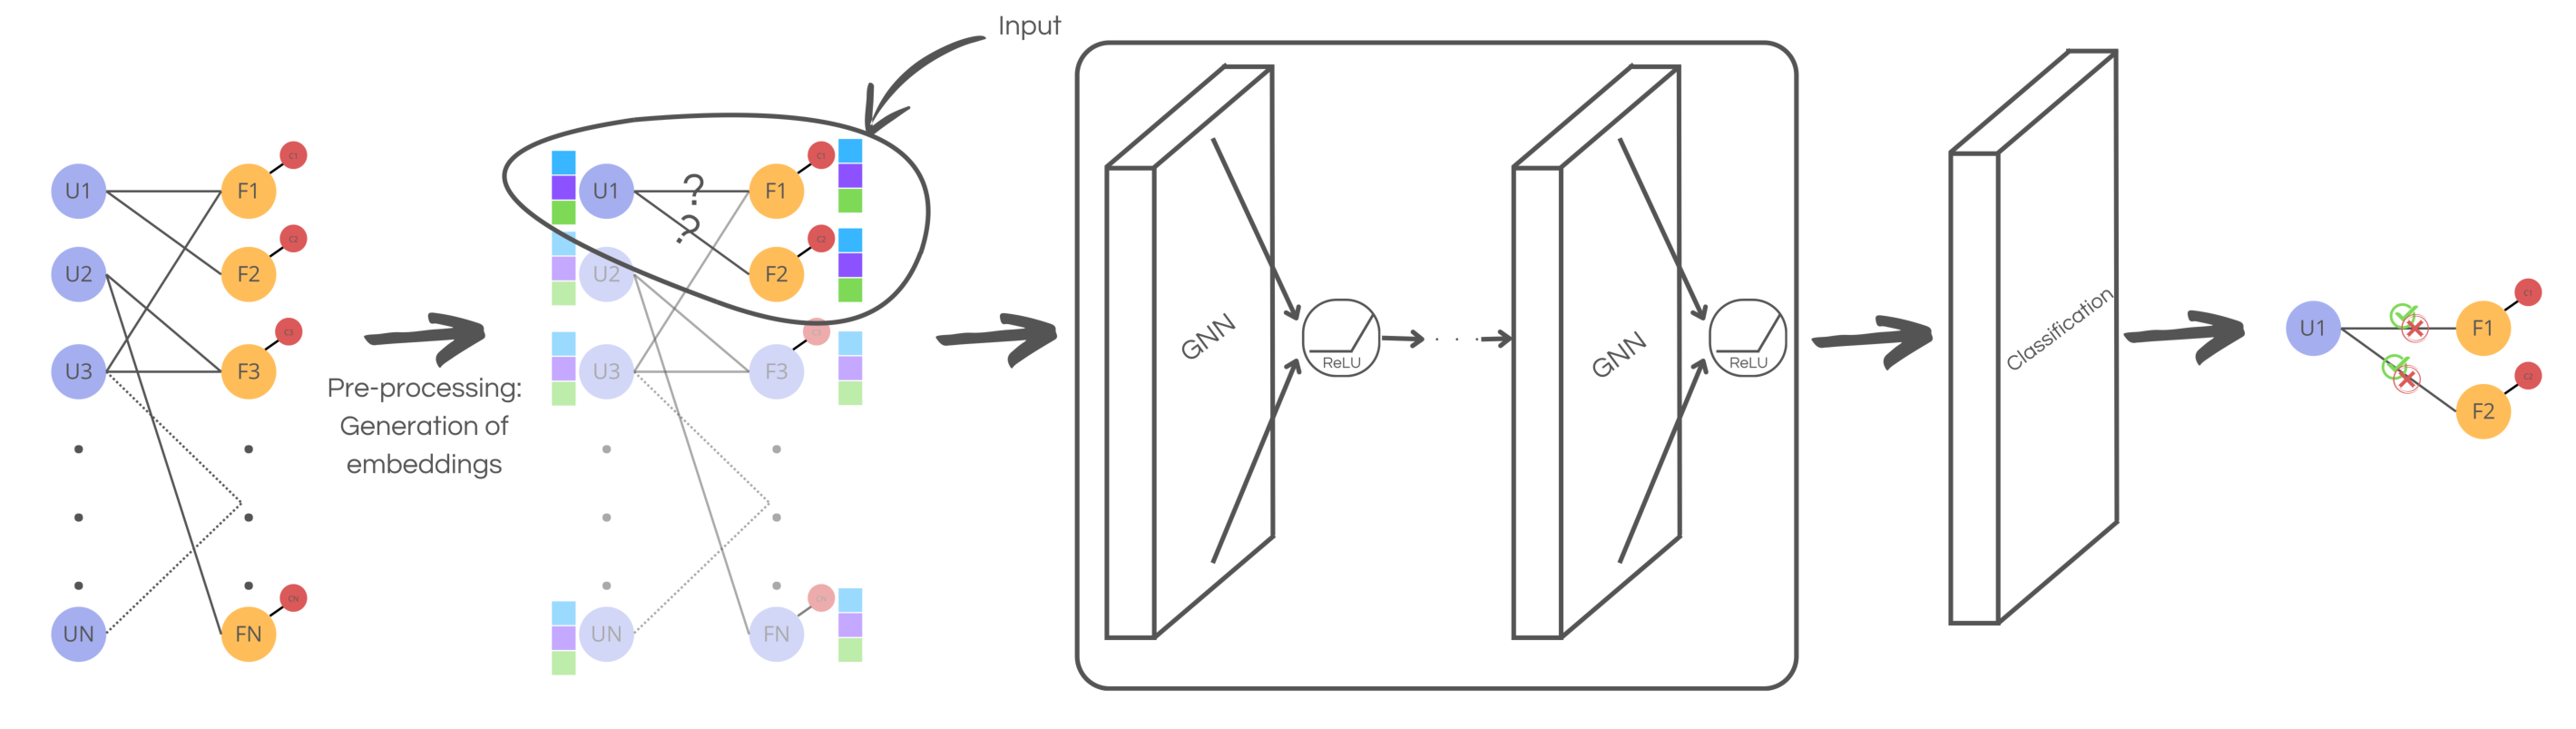
\includegraphics[width=1\linewidth]{figures/architecture.pdf}

  \caption{
    Architecture
  }
  \label{fig:architecture}
\end{figure*}

\section{Experimental setup}\label{sec:experimental-setup}

\paragraph{Dataset exploration}

\paragraph{Text cleaning}

\subsection{Model configuration}\label{sec:model-config}

\paragraph{Encoder}


\paragraph{Decoder}



\subsection{Training process}\label{sec:training-process}

\bibliography{bibliography}


% \appendix

% \section{Example Appendix}
% \label{sec:appendix}

% This is an appendix.

\end{document}
